\chapter{Topological Band Structure Theory}

Last session closed on the honeycomb lattice's most striking feature: near the corners of its
Brillouin zone, the tight-binding band structure stops looking parabolic and becomes linear, the
Dirac cone, one of the three dispersion archetypes (parabolic, Dirac, flat) that we singled out as
organizing the rest of the course. We even saw that this is not just a theorist's convenience: ARPES
measures that linear dispersion directly in real graphene. So here is the question that organizes
today's entire session: what happens if we open a gap at that Dirac point? A gapped Dirac cone turns
a metal into an insulator, but not always an ordinary one. Depending on exactly \emph{how} the gap opens,
the resulting insulator can carry a hidden invariant, a topological invariant, that shows up nowhere
in the bulk spectrum itself but forces the material to have conducting states at its edge, states
that no local disorder can remove. Getting to that statement rigorously is going to take some work:
we need linear response theory as a tool, the Hall conductivity as the observable that first reveals
the invariant, the Chern number as the invariant itself, and the general bulk-boundary correspondence
that ties the invariant to edge physics. We will build all of this using the quantum Hall state as
the simplest possible example, then bring the same machinery back to a purely one-dimensional model
(the SSH chain) before finally returning, in Section 3.10, to gap open the honeycomb Dirac cone
itself and see a genuine Chern insulator emerge with no magnetic field anywhere in sight.

\section{What topological materials are}

Before diving into formalism it is worth having a rough taxonomy in view, so that the abstract
machinery we are about to build has concrete targets to attach to. Topological materials, as a
class, are systems with an excitation gap in the bulk that simultaneously host protected excitations
at their surface or edge. That combination, gapped bulk plus gapless boundary, is going to recur
throughout the session, and it is genuinely the defining feature: it is not that the edge happens to
have low-energy states, it is that the bulk topology \emph{forces} them to be there.

Within that class we will meet, over today and the following session:

\begin{itemize}
\item The \textbf{quantum Hall effect}, realized in two-dimensional electron gases and in graphene under a
  strong perpendicular magnetic field; the simplest topological state, and our starting point.
\item The \textbf{quantum anomalous Hall effect}, the same physics without any external magnetic field at
  all, which we will construct explicitly in Section 3.10.
\item \textbf{Quantum spin Hall insulators}, effectively two time-reversed copies of a quantum Hall state
  glued together (Section 3.11).
\item \textbf{Topological superconductors}, whose surface excitations are Majorana modes, and which underlie
  one route to topological quantum computing (we return to these in full in session 5).
\item \textbf{Topological semimetals}, including Weyl semimetals, whose low-energy quasiparticles are Weyl
  fermions.
\item \textbf{Topological Kondo insulators}, this year's spoken example of topology surviving in a strongly
  correlated, many-body setting, ``and many others that do not fit on this slide.''
\end{itemize}

This is slide-only material with no notebook counterpart: the slides name specific material
realizations for each entry (graphene for the quantum Hall effect, Cr-doped (Bi,Sb)$_2$Te$_3$ for
the quantum anomalous Hall effect, Bi$_2$Se$_3$ for the quantum spin Hall effect, Fe chains on Pb for
a topological superconductor, TaAs for a Weyl semimetal, and SmB$_6$ for its many-body example) that
were shown but not narrated in detail, and the course's notebook does not simulate any of these
specific compounds: the taxonomy slide's many-body example is the topological Kondo insulator,
with SmB$_6$ as the material realization. What we will simulate, in the models
built up over this session, are minimal tight-binding versions of the first three items on the list
above.

\section{Linear response theory: how a measurement reads off the wavefunctions}

To see why a bulk band structure can carry an invariant at all, we need a tool for connecting the
wavefunctions of a Hamiltonian to something we can actually measure. That tool is linear response
theory, and the idea behind it is completely general: perturb the system at some position $x$ and
time $t$, then measure some observable, charge, current, magnetization, heat, at another position
$x'$ and time $t'$. Linear response theory tells us that this measured response depends only on the
electronic structure of the unperturbed material.

Two examples make this concrete before we specialize to the Hall conductivity. Put an impurity into
a two-dimensional metal and look at how the electron density, or the local density of states, gets
modulated around it: linear response theory shows that this modulation pattern (the Friedel
oscillation) directly encodes the Fermi wavelength of the electron gas, which is exactly what
scanning tunneling microscopy exploits in practice. Similarly, scattering neutrons off a magnetic
material lets the neutron's magnetic moment couple to the local moments in the sample; the resulting
scattering pattern reconstructs both the magnetic structure and its excitations, in particular
magnons. Both of these are slide-only illustrations in the sense that the labeled Friedel-oscillation
and neutron-scattering figures were shown on screen without being narrated in full; the physical
content of both examples, however, was explained in speech and is worth keeping in mind as the
general payoff of the formalism we build next.

Formally, we start from an unperturbed Hamiltonian $H_0$ and add a perturbation controlled by a
dimensionless parameter $\lambda$,

\begin{equation*}
H(\lambda) = H_0 + \lambda V,
\end{equation*}

so that $\lambda = 0$ recovers the original system and $\lambda = 1$ is the fully perturbed one. Any
observable, the energy, the density, the magnetic moment, the current, or the wavefunctions
themselves, can then be Taylor-expanded in $\lambda$; the derivative of an observable with respect to
$\lambda$ at $\lambda = 0$ is what we call the response of the system (its susceptibility, in the
case of a magnetic perturbation). Since every observable can be built from the wavefunctions, the
most useful object to expand is the ground-state wavefunction itself. For a state $|n\rangle$ of the
unperturbed Hamiltonian $H_0$ with energy $\varepsilon_n$, standard first-order perturbation theory
gives

\begin{equation}
|n\rangle_\lambda = |n\rangle + \lambda \sum_{m \neq n} \alpha_m\, |m\rangle + \mathcal{O}(\lambda^2),
\qquad \alpha_m = \frac{\langle m|V|n\rangle}{\varepsilon_n - \varepsilon_m}.
\end{equation}

Everything that follows today, the Hall conductivity, the Berry curvature, the Chern number, comes
directly from plugging (3.1) into the definition of some observable.

\section{Where perturbation theory breaks down}

Before using (3.1), it is worth being honest about when it fails, because several of the most
important phenomena in this course live exactly in that failure. The expansion (3.1) implicitly
assumes we are in the \emph{perturbative regime}: a small change in the input (the perturbation strength)
produces a small change in the output. This is not automatic. Three cases are worth naming now,
because we will meet each one properly later in the course:

\begin{itemize}
\item An impurity placed in a metal produces the \textbf{orthogonality catastrophe}: the many-body ground
  state after the perturbation becomes exactly orthogonal to the original ground state, however
  small the perturbation, so no finite-order Taylor expansion in $\lambda$ can connect the two.
\item A quantum spin (a local magnetic moment) coupled to a metal produces the \textbf{Kondo effect}: the
  relevant energy scale, the Kondo temperature, is a non-perturbative function of the coupling
  constant, and no order of perturbation theory in that coupling reproduces it. We will meet the
  Kondo lattice model properly in session 8; today's mention is a first flag that ordinary
  perturbation theory has a hard limit.
\item \textbf{Superconductivity} is likewise non-perturbative: the BCS gap does not appear at any finite order
  in the interaction strength starting from the normal state. Session 5 works this out in full.
\end{itemize}

For today's lecture, and for every model we build in this session, we stay safely inside the regime
where (3.1) holds. It is enough, for now, to know that it does not always.

\section{The Hall conductivity from linear response}

Now we specialize (3.1) to the measurement that is going to carry us to topology: the transverse, or
Hall, conductivity. Take a two-dimensional material, apply a voltage in the $y$ direction, and ask
what current flows in the $x$ direction. In momentum space, a voltage in $y$ enters as a perturbation
proportional to $\partial H/\partial k_y$ (it shifts $k_y$ via the Peierls substitution), and the
current operator in the $x$ direction is, up to the electron charge, the group-velocity operator
$\partial H/\partial k_x$. Both are exactly the kind of matrix element that (3.1) hands us.

Substituting (3.1) into the definition of the Hall conductivity gives an expression built from two
velocity operators and an energy denominator, the standard Kubo formula for a filled band $n$ and
empty bands $m$,

\begin{equation}
\sigma_{xy} \;\propto\; \sum_{n\ \text{filled}} \sum_{m\ \text{empty}} \int_{\text{BZ}}
\frac{d^2k}{(2\pi)^2}\;
\frac{\langle n|\partial_{k_x}H|m\rangle\langle m|\partial_{k_y}H|n\rangle - (x\leftrightarrow y)}
{(\varepsilon_n - \varepsilon_m)^2}.
\end{equation}

At this point the expression still depends explicitly on the band energies through the denominator,
which looks like it should depend on all the messy details of the band structure. It does not, and
seeing why is the whole point of the next section.

\section{The Berry curvature, and why the Hall conductivity is an integer}

Differentiate the Schrödinger equation $H(k)|u_n(k)\rangle = \varepsilon_n(k)|u_n(k)\rangle$ with
respect to $k_\mu$ and project onto a different band $\langle u_m(k)|$, $m \neq n$:

\begin{equation}
\langle u_m|\partial_{k_\mu} H|u_n\rangle
= \big(\varepsilon_n(k) - \varepsilon_m(k)\big)\,\langle u_m|\partial_{k_\mu} u_n\rangle.
\end{equation}

This identity is exactly the piece we need: it trades a matrix element of $\partial_k H$ for a matrix
element of the wavefunction's own $k$-derivative, divided by the energy difference. Using (3.3) to
rewrite the numerator and denominator of (3.2) together, the explicit energy dependence cancels
completely, and what remains is an object built purely from wavefunction overlaps, the \textbf{Berry
curvature} of band $n$,

\begin{equation*}
\Omega_n(k) = -2\,\mathrm{Im}\, \langle \partial_{k_x} u_n(k)|\partial_{k_y} u_n(k)\rangle,
\end{equation*}

so that the Hall conductivity of a set of filled bands is

\begin{equation}
\sigma_{xy} = \frac{e^2}{h}\, C, \qquad
C = \sum_{n\ \text{filled}} \frac{1}{2\pi}\int_{\text{BZ}} \Omega_n(k)\, d^2k.
\end{equation}

This is the central result of the session. Two things about (3.4) deserve emphasis. First, $\sigma_{xy}$
depends only on how the wavefunctions vary across the Brillouin zone, not on the energies at all: you
can deform the band structure however you like, and as long as the wavefunctions do not change,
the Hall conductivity is untouched. Second, and more strikingly, for a gapped (insulating) system $C$
is always an integer, regardless of how many bands are involved or what the dispersion looks like.
This is a genuinely topological statement: the Brillouin zone of a two-dimensional system is a
compact manifold (a torus, since opposite edges of the zone are identified), and integrating a
curvature over a closed surface always produces an integer, exactly as it does for the Gaussian
curvature of an ordinary closed surface in differential geometry. This integer $C$ is the \textbf{Chern
number}, and (3.4) is the first place in the course where a measurable quantity, the Hall
conductivity, is pinned to a topological invariant.

\section{The quantum Hall state: Landau levels and chiral edge states}

The Chern number appears in its cleanest form in the quantum Hall state itself: a two-dimensional
electron gas in a strong perpendicular magnetic field. The resulting band structure is exactly the
flat-band archetype from session 2, a set of dispersionless Landau levels, and each Landau level
individually carries Chern number $+1$. Filling the first Landau level gives total Chern number $C=1$;
filling the first two gives $C=2$; and so on, so that $\sigma_{xy} = C\, e^2/h$ steps through
successive integer plateaus as the chemical potential is raised through successive Landau levels.
This is the integer quantum Hall effect, and session 4 works out its full phenomenology (including
the fractional generalization); today we only need the Chern-number bookkeeping.

Here is the puzzle this raises. We have an insulator (a gap between Landau levels), yet $\sigma_{xy}$
is a \emph{conductivity}, meaning some electron somewhere has to be moving. The resolution is that any
real sample has an edge, and at that edge the bulk gap closes: gapless edge states appear, carrying
exactly the current that (3.4) predicts. These edge states have a further, crucial property: on a
given edge, states propagate in only \emph{one} direction. The top edge of a sample carries current one
way and only that way; the bottom edge carries it the opposite way and only that way. A mode that
propagates in a single direction is called \textbf{chiral}, and chirality is precisely what protects the
quantum Hall state against disorder: an electron in a chiral edge mode has nowhere to backscatter
into, since there is no counter-propagating state at the same edge and energy to scatter into. No
backscattering channel means no resistance in that channel. Figure~\ref{fig:s03:chiraledge} shows
both halves of this picture: the closed bulk orbits that carry nothing, the skipping orbits that
carry everything, and what happens when an impurity is put in their way.

% Session 3 -- why an "insulator" conducts: chiral edge states in real space.
% Placement: sec. "The quantum Hall state", after the chirality/backscattering
% paragraph; referenced again from the robustness paragraph of sec. 3.7.
%
% LAYOUT NOTE: pure tikzpicture, bare canvas coordinates throughout.
%
% SIGN CONVENTION, checked against the semiclassical drift: electrons (charge
% -e) in a field B out of the page orbit counter-clockwise in the bulk, and the
% confining potential at the boundary gives an E x B drift of +x along the top
% edge and -x along the bottom edge. The edge circulation is therefore
% clockwise, i.e. opposite in sense to the bulk cyclotron motion. Reversing B
% reverses every arrow in the figure at once.
\begin{aqmfigure}{fig:s03:chiraledge}{Chiral edge states, and why they cannot be backscattered.
(a) A quantum Hall sample. In the bulk the electrons move on closed cyclotron orbits and do not go
anywhere, and the system is an insulator with a gap between Landau levels. At the boundary these
orbits cannot close. They skip along the edge, and for a given direction of $B$ they skip in one
direction only, which is opposite on the two edges. Propagation in a single direction is what the
word \textbf{chiral} means, and it carries the current that $\sigma_{xy}=C\,e^2/h$ predicts, even
though the bulk is gapped. (b) The consequence. An impurity at the edge can deflect the mode, but
there is no state that propagates in the opposite direction at the same edge and the same energy for
it to scatter \emph{into}, so the mode goes around the obstacle and continues. Without a
backscattering channel there is no resistance, which is why the Hall plateaus are quantized so
sharply. If we reverse the sign of $B$, all the arrows are reversed at the same time.}

\begin{tikzpicture}[x=1cm, y=1cm]

% =====================================================================
% (a) the sample
% =====================================================================
\def\W{7.2}
\def\Ht{3.9}

\node[aqmpanel, anchor=south west] at (0,\Ht+1.02) {(a) a gapped bulk with conducting edges};

% sample body
\fill[aqmfill] (0,0) rectangle (\W,\Ht);
\draw[aqm, draw=black] (0,0) rectangle (\W,\Ht);

% --- bulk: closed cyclotron orbits (counter-clockwise) ---------------
\foreach \a/\b in {1.00/2.95, 2.60/3.05, 4.30/2.95, 5.90/3.05,
                   6.60/1.95, 3.60/0.95, 5.30/0.95, 6.60/0.95, 1.00/1.95} {
  \draw[aqm, draw=aqmaccent, line width=0.8pt] (\a,\b) circle (0.30);
  \draw[aqm, draw=aqmaccent, -{Stealth[length=4.5pt,width=3.6pt]}, line width=0.8pt]
    ($ (\a,\b) + (-18:0.30) $) arc (-18:22:0.30);
}

% magnetic field symbol
\node[circle, draw=black, fill=white, line width=\aqmthinwidth,
      minimum size=11pt, inner sep=0pt] at (0.62,0.95) {};
\fill[black] (0.62,0.95) circle (1.1pt);
\node[aqmlabsmall, anchor=west] at (0.88,0.95) {$B$ out of page};

\node[aqmlabsmall, align=center, fill=aqmfill, inner sep=2pt]
  at (3.80,1.95)
  {\textbf{bulk:} closed cyclotron orbits,\\[-1pt] gapped, no net transport};

% --- top edge: skipping orbits drifting to the right -----------------
\foreach \i in {0,1,...,9} {
  \draw[aqm, draw=aqmbroken, line width=1.0pt]
    ({0.40+\i*0.66},\Ht) arc (180:360:0.33);
}
\foreach \i in {1,4,7} {
  \draw[aqm, draw=aqmbroken, -{Stealth[length=5.5pt,width=4.4pt]}, line width=1.0pt]
    ($ ({0.73+\i*0.66},\Ht) + (250:0.33) $) arc (250:292:0.33);
}
\draw[aqm, draw=aqmbroken, -{Stealth[length=6pt,width=5pt]}, line width=1.3pt]
  (1.7,\Ht+0.32) -- (5.5,\Ht+0.32);
\node[aqmlabsmall, anchor=south, text=aqmbroken] at (3.6,\Ht+0.40)
  {top edge: right-movers only};

% --- bottom edge: skipping orbits drifting to the left ---------------
\foreach \i in {0,1,...,9} {
  \draw[aqm, draw=aqmbroken, line width=1.0pt]
    ({0.40+\i*0.66},0) arc (180:0:0.33);
}
\foreach \i in {1,4,7} {
  \draw[aqm, draw=aqmbroken, -{Stealth[length=5.5pt,width=4.4pt]}, line width=1.0pt]
    ($ ({0.73+\i*0.66},0) + (68:0.33) $) arc (68:110:0.33);
}
\draw[aqm, draw=aqmbroken, -{Stealth[length=6pt,width=5pt]}, line width=1.3pt]
  (5.5,-0.32) -- (1.7,-0.32);
\node[aqmlabsmall, anchor=north, text=aqmbroken] at (3.6,-0.40)
  {bottom edge: left-movers only};

% --- side edges close the loop ---------------------------------------
\draw[aqm, draw=aqmbroken, -{Stealth[length=6pt,width=5pt]}, line width=1.3pt]
  (\W+0.32,\Ht-0.7) -- (\W+0.32,0.7);
\draw[aqm, draw=aqmbroken, -{Stealth[length=6pt,width=5pt]}, line width=1.3pt]
  (-0.32,0.7) -- (-0.32,\Ht-0.7);

% =====================================================================
% (b) an impurity at the edge
% =====================================================================
\begin{scope}[xshift=8.9cm, yshift=1.50cm]

\node[aqmpanel, anchor=south west] at (0,2.94) {(b) an impurity cannot stop it};

\fill[aqmfill] (0,0.10) rectangle (5.4,1.80);
\draw[aqm, draw=black] (0,1.80) -- (5.4,1.80);
\node[aqmlabsmall, anchor=south west, text=aqmmuted] at (0.06,1.90) {vacuum};
\node[aqmlabsmall, anchor=north west, text=aqmmuted] at (0.06,1.38) {sample};

% the impurity
\node[circle, draw=black, fill=aqmmuted, line width=\aqmthinwidth,
      minimum size=15pt, inner sep=0pt] at (2.70,1.68) {};
\node[aqmlabsmall, anchor=south west] at (2.98,1.98) {impurity};
\draw[aqm, draw=black, line width=\aqmthinwidth] (2.86,1.86) -- (3.02,2.02);

% the rerouted chiral mode
\draw[aqm, draw=aqmbroken, line width=1.3pt, -{Stealth[length=6pt,width=5pt]}]
  (0.85,1.52) -- (1.90,1.52)
  .. controls (2.34,1.52) and (2.26,0.95) .. (2.70,0.95)
  .. controls (3.14,0.95) and (3.06,1.52) .. (3.50,1.52)
  -- (5.10,1.52);
\node[aqmlabsmall, anchor=west, text=aqmbroken, align=left] at (3.30,0.92)
  {reroutes and\\[-1pt]carries on};

% the forbidden backscattering channel
\draw[aqm, draw=aqmmuted, line width=1.0pt, dash pattern=on 3pt off 2pt,
      -{Stealth[length=5pt,width=4pt]}] (2.90,0.45) -- (1.05,0.45);
\draw[aqm, draw=aqmbroken, line width=1.3pt] (1.75,0.24) -- (2.20,0.66);
\draw[aqm, draw=aqmbroken, line width=1.3pt] (1.75,0.66) -- (2.20,0.24);
\node[aqmlabsmall, anchor=north, align=center, text width=6.6cm] at (2.70,-0.06)
  {no counter-propagating state at this edge and this energy:
   the impurity has nothing to scatter into};

\end{scope}

\end{tikzpicture}

\end{aqmfigure}


A concrete model makes this vivid: a tight-binding square lattice with a perpendicular magnetic
field, cut into a finite-width ribbon (translationally invariant along the ribbon but finite across
it). Diagonalizing this ribbon shows exactly the structure just described: flat, Landau-level-like
bulk bands, plus dispersive edge branches crossing the gap, one branch confined to each edge and
propagating in only one direction. Zooming into the low-energy region near zero energy, the level
spacing between the flat bands approaches the familiar equal spacing of a continuum two-dimensional
electron gas in a magnetic field, so the tight-binding model smoothly reproduces the textbook Landau
problem in the appropriate limit. This particular computed band-structure figure (bulk flat bands in
green plus the two counter-propagating edge branches) is shown on the slides but only described
qualitatively in speech; reproducing it numerically is exactly what the notebook callout below asks
you to do.

\begin{notebookbox}{\texttt{session3.ipynb}, ``From electrons in a ribbon to the quantum Hall state'' (Core), ``The quantum Hall effect in graphene'' (Core), and ``Localization of the edge states in the quantum Hall effect'' (Challenge)}
Build a square-lattice (then honeycomb-lattice) ribbon with a magnetic field and reproduce the
figure described above: flat Landau-level bulk bands plus chiral edge branches. Check the
propagation direction of the edge states at positive versus negative energy on each edge, exactly
the chirality argument of Section 3.6, then look at how the edge states localize in real space as
a function of energy and how that localization responds to a weaker field or a narrower ribbon.
\end{notebookbox}

\section{What ``topology'' means for a Hamiltonian, and the bulk-boundary correspondence}

We have now seen one topological invariant in action; it is worth stepping back and saying what
``topological'' actually means, in the mathematical sense the word is borrowed from. Topology
classifies objects by whether they can be smoothly deformed into one another without a drastic
operation, cutting, tearing, gluing. Three-dimensional surfaces are classified by their number of
holes: a donut and a coffee cup both have exactly one hole and can be continuously deformed into each
other, while a sphere has none and cannot be deformed into either. Closed curves in one dimension
have an analogous classification by knots: curves with inequivalent knots cannot be smoothly
untangled into one another.

For a Hamiltonian, the analogous ``deformation'' is changing the band structure continuously while
keeping the bulk gap open. Two Hamiltonians related by such a deformation share the same Chern
number, precisely because $C$ in (3.4) is quantized and therefore cannot change continuously; it can
only jump, and a jump requires the gap to close at some point along the deformation. So the Chern
number plays the role that the number of holes plays for a surface: Hamiltonians with the same Chern
number are topologically equivalent (deformable into each other without closing the gap), and
Hamiltonians with different Chern numbers are not.

This has an immediate and powerful consequence. Suppose we build a spatially varying Hamiltonian that
equals $H_1$ (Chern number $C_1$) far to the left and $H_2$ (Chern number $C_2 \neq C_1$) far to the
right. Since $H_1$ and $H_2$ cannot be deformed into each other without closing the gap, and the
interpolating Hamiltonian passes continuously from one to the other, the gap \emph{must} close somewhere
in between, irrespective of how the interface is actually constructed microscopically. This is the
\textbf{bulk-boundary correspondence}: an interface between two bulk phases with different Chern numbers
always hosts a gapless state, and that gapless state's existence depends only on $C_1$ and $C_2$, not
on any detail of the interface. The vacuum itself has $C=0$ (it is, trivially, topologically trivial),
so a quantum Hall state with $C=1$ automatically has a gapless edge state at every boundary with
vacuum, which is exactly the edge physics of Section 3.6 recovered from a completely general argument.
Figure~\ref{fig:s03:bulkboundary} sets out the three steps of that argument in order.

% Session 3 -- the bulk-boundary correspondence: an integer that has to jump
% Placement: sec. "What topology means for a Hamiltonian", after the
% interpolating-Hamiltonian paragraph.
% Rendered by figures/blender/s03f02_bulkboundary.py, labels in figures/overlays/s03f02_bulkboundary.tex.
\begin{aqmfigure}{fig:s03:bulkboundary}{The bulk-boundary correspondence, as an argument about an
integer. A Hamiltonian changes slowly in space from $H_1$ on the left to $H_2$ on the right, which
is the color of the backdrop. In the top row, the Chern number is an integer, so it cannot change
continuously from $C_1=1$ to $C_2=0$ and it can only jump. In the middle row, a jump is only allowed
where the quantization argument itself fails, which is where the gap closes, so the local gap must
go to zero somewhere in the interface region, at the cross. This is drawn schematically, in the
local-gap approximation. In the bottom row, the state that appears there is a gapless state bound to
the interface. This argument does not use any detail of how the interface is built, and only $C_1$
and $C_2$ enter, which is why the edge state survives rough boundaries and impurities. If we take
$H_2$ to be the vacuum, $C_2=0$, we obtain the chiral edge state of figure~\ref{fig:s03:chiraledge}
from a completely general argument.}
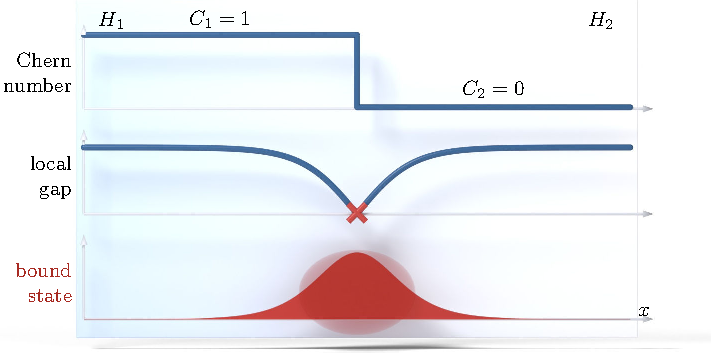
\includegraphics{figures/pdf/s03f02_bulkboundary.pdf}
\end{aqmfigure}


The same argument explains the robustness we already invoked. Introduce a local impurity at the edge
of a quantum Hall sample: this only changes the microscopic details of the vacuum/quantum-Hall
interface, and since the interface's topological excitation must exist regardless of those details,
the edge state simply reconstructs itself around the impurity rather than being scattered by it. This
is the general mechanism, not special to the quantum Hall case, and it will reappear for every
topological invariant we meet from here on.

\section{Three topological material classes}

With the general machinery in place, three classes of topological matter are worth naming before we
build explicit models for two of them:

\begin{itemize}
\item \textbf{Chern insulators}: bulk Chern number $C \neq 0$, chiral edge states, and time-reversal symmetry
  necessarily broken (we will see in Section 3.11 that time-reversal symmetry forces $\sigma_{xy}=0$).
  No backscattering channel means no electrical losses at the edge, which makes them an attractive
  platform for dissipationless electronics.
\item \textbf{Quantum spin Hall insulators}: two copies of a Chern insulator, one per spin, with opposite
  Chern number, so the net Chern number vanishes and time-reversal symmetry is preserved, but the
  edge states are \textbf{helical}: spin-up and spin-down propagate in opposite directions along the same
  edge. This is the natural platform for dissipationless spin transport, i.e. spintronics.
\item \textbf{Topological superconductors}: a bulk superconducting gap combined with gapless surface
  excitations that are their own antiparticle, Majorana excitations. Because the corresponding
  quantum information is stored non-locally, conventional local decoherence channels do not act on
  it directly, which is the basis of topological quantum computing. We build the minimal model for
  this case, the Kitaev chain, in session 5, and we will see there that it is literally the same
  model as the one we are about to construct next.
\end{itemize}

\section{The SSH model: a minimal one-dimensional topological insulator}

We now build the simplest possible model that shows this physics explicitly: the Su-Schrieffer-Heeger
(SSH) chain. It looks almost too simple to be useful, but it is worth taking seriously, not least
because the simplest model for a topological superconductor, the Kitaev chain, turns out to be
exactly this model written in Majorana language.

Take a one-dimensional lattice with two sites per unit cell, $A$ and $B$, and two hopping amplitudes:
an intracell hopping $t$ (within a unit cell) and an intercell hopping fixed at $1$ (between
neighboring unit cells). Consider first the extreme limit in which the intracell hopping dominates,
$t \gg 1$, so that the chain is fully dimerized with alternating bonds: strong bonds of strength $t$
coupling sites $(0,1)$, $(2,3)$, $(4,5)$, \ldots and negligible coupling between $(1,2)$, $(3,4)$,
\ldots. Each dimer is then an isolated two-level system with
bonding and antibonding eigenstates at energies $\pm t$; the whole chain's spectrum is just this pair
of levels repeated once per dimer, and there is nothing at zero energy.

Now take the opposite limit, $t \to 0$, in which the strong bonds are the intercell ones and the
dimerization pattern is shifted by one site: leave the very first site uncoupled (a ``dangling''
site), couple $(1,2)$, $(3,4)$, \ldots, and leave the very last site dangling as well. In the bulk this
looks identical to the previous chain (the same alternating dimer pattern, just shifted by one site),
but the two ends are qualitatively different: each end now hosts a genuinely uncoupled site.
Diagonalizing this chain gives the analogous bonding/antibonding pairs at $\pm 1$ in the bulk, plus
\textbf{two states pinned exactly at zero energy}, one localized at each end. Figure~\ref{fig:s03:ssh}
shows the two chains side by side together with the spectra they produce.

% Session 3 -- the SSH chain: the same bulk, two dimerizations, two spectra.
% Placement: sec. "The SSH model", after the dangling-site paragraph.
% Rendered by figures/blender/s03f03_ssh.py, labels in figures/overlays/s03f03_ssh.tex.
\begin{aqmfigure}{fig:s03:ssh}{The Su-Schrieffer-Heeger chain, drawn with the same eight sites and
the same unit cells in both rows, which are the translucent slabs, so that the only difference is
which of the two bonds is the strong one, drawn as the thick rod. Next to each chain is its
spectrum, the eigenvalues of the open chain in units of the strong hopping. (a) In front, the
intracell hopping dominates, $t\gg1$ (here $t=4$). Every site is paired into a dimer, and the levels
form two groups around $\pm t$, spread a little by the weak hopping, with a clear gap around zero,
which is the trivial phase. (b) Behind, the intercell hopping dominates, $t\to0$ (here $t=1/4$). The
dimer pattern is shifted by one site and the first and last sites, the two glowing ones, are left
uncoupled. The same bulk spectrum now has two extra states at $E=0$, the two short rods in the gap,
one localized at each end, which is the topological phase. The two chains cannot be distinguished
in the bulk, and the difference is only at the ends, which is what a bulk invariant has to predict.
At small but finite $t$ the two end states hybridize through the chain, and their splitting away
from zero is only exponential in the chain length. For $t=1/4$ and eight sites the two levels sit
at $\pm0.004$, which is too small to see at this scale.}
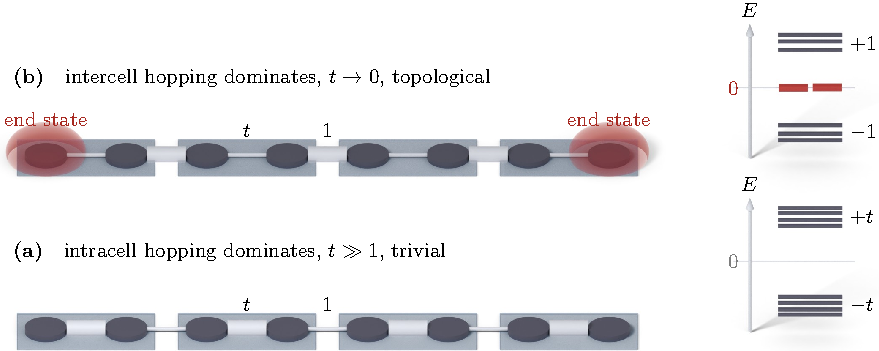
\includegraphics{figures/pdf/s03f03_ssh.pdf}
\end{aqmfigure}


This is the minimal example of a topological phase. The fully dimerized chain (first case) is the
\textbf{trivial phase}: gapped everywhere, including at the ends. The shifted chain (second case) is the
\textbf{topological phase}: gapped in the bulk, but with gapless, exactly-zero-energy modes at the edges.
It looks like a very fine-tuned construction, and it is; real chains have hopping between every pair
of neighboring sites. What survives fine-tuning is the important part: turning on a small coupling
$t$ between the originally-decoupled sites at the two ends does \emph{not} remove the zero modes, as long
as $t$ stays below the bulk hopping strength. Intuitively, for $t \ll 1$ we are weakly coupling an
isolated zero-energy level to a gapped bulk, and a weak coupling cannot push a level all the way
across a finite gap. More rigorously, this is exactly the deformation argument of Section 3.7: the
Hamiltonians at different small $t$ are topologically equivalent, connected without closing the bulk
gap, so whatever invariant protects the zero mode at $t=0$ continues to protect it.

We can make this fully precise using the Bloch Hamiltonian. With intracell hopping $t$ and intercell
hopping normalized to $1$, the momentum-space Hamiltonian in the $(A,B)$ basis is the $2\times 2$
matrix

\begin{equation}
H(k) = \begin{pmatrix} 0 & d(k) \\ d^*(k) & 0 \end{pmatrix}
= (t + \cos k)\,\sigma_x + \sin k\,\sigma_y, \qquad d(k) = t + e^{ik},
\end{equation}

with eigenvalues $E_\pm(k) = \pm|d(k)| = \pm\sqrt{1 + t^2 + 2t\cos k}$. The gap closes exactly when
$d(k)=0$, which requires $t=1$ and $k=\pi$: this is the topological phase transition point, and it
matches the qualitative $t<1$ versus $t>1$ split above, since at $t=0$ the chain is the fully
dangling-site (topological) limit and at $t=1$ it becomes the fully symmetric, gapless chain.

The topological invariant here is the \textbf{Zak phase}, the one-dimensional Berry phase accumulated by
the lower-band Bloch state $|u_-(k)\rangle$ as $k$ sweeps once around the Brillouin zone,

\begin{equation}
\gamma = i \oint_{\text{BZ}} \langle u_-(k)|\partial_k u_-(k)\rangle\, dk \pmod{2\pi}.
\end{equation}

Geometrically, $\gamma/\pi$ counts how many times $d(k)$ winds around the origin as $k$ runs from $0$
to $2\pi$; from (3.5), $d(k) = t + e^{ik}$ traces a unit circle centered at $(t,0)$ in the complex
plane. That circle encloses the origin exactly when $|t|<1$, and does not when $|t|>1$: consistent
with everything above, $\gamma = \pm\pi$ (one winding, a topological insulator, gapless edge modes)
for $t<1$, and $\gamma = 0$ (no winding, a trivial insulator, no edge modes) for $t>1$. The value of
the Zak phase is in exact one-to-one correspondence with the presence or absence of a zero-energy
edge state: this is the one-dimensional version of the bulk-boundary correspondence from Section 3.7.
Figure~\ref{fig:s03:winding} draws that winding together with the bands it controls, and makes the
point that the two insulating phases are indistinguishable in their spectra alone.

% Session 3 -- the SSH invariant made visible: the winding of d(k)=t+e^{ik}.
% Placement: sec. "The SSH model", after equation (3.6) (the Zak phase).
%
% LAYOUT NOTE: every annotation lives inside its own axis and is placed in
% "axis cs:" coordinates. The complex-plane panels use "scale only axis" with
% identical x- and y-ranges so that the circles come out round.
\begin{aqmfigure}{fig:s03:winding}{A drawing of the one-dimensional invariant. The top row shows the
off-diagonal element $d(k)=t+e^{ik}$ of the SSH Bloch Hamiltonian (3.5) in the complex plane, as $k$
goes once through the Brillouin zone, and the arrow shows the direction of increasing $k$. It is
always the unit circle, but centred at $(t,0)$, so it encloses the origin for $t<1$ and does not
enclose it for $t>1$. The winding number of this curve around the origin is exactly $\gamma/\pi$,
which is the Zak phase (3.6) in units of $\pi$. The bottom row shows the corresponding bands
$E_\pm(k)=\pm|d(k)|$, with gap $2|1-t|$. The two rows give the same information in two ways. The only
way to unwind the curve is to move it across the origin, and $d(k)=0$ is where the gap closes, so the
invariant cannot change while the system stays insulating. Note that (a) and (c) have the same gap
and look like ordinary spectra. The difference between them cannot be seen in the energies and is
only in the wavefunctions, which is the main point of (3.4). By the bulk-boundary correspondence,
$\gamma=\pi$ is also exactly the condition for the zero-energy end modes of
figure~\ref{fig:s03:ssh}.}

\begin{tikzpicture}

% =====================================================================
% top row: d(k) in the complex plane. Columns at x = 0, 5.3, 10.6 cm.
% =====================================================================

% ---------- (a) t = 0.5 : winding 1 ----------------------------------
\begin{axis}[
  aqmplot, scale only axis, width=3.5cm, height=3.5cm,
  at={(0cm,0cm)}, anchor=north west,
  axis lines=middle,
  xmin=-1.45, xmax=2.85, ymin=-2.15, ymax=2.15,
  xtick={1,2}, ytick={1},
  xlabel={$\mathrm{Re}\,d$}, ylabel={$\mathrm{Im}\,d$},
  xlabel style={at={(axis description cs:1.03,0.5)}, anchor=west, font=\footnotesize},
  ylabel style={font=\footnotesize},
  title={(a) $t=0.5$},
]
\addplot[aqmcurve, domain=0:360, samples=90] ({0.5+cos(x)},{sin(x)});
\draw[aqm, draw=aqmaccent, -{Stealth[length=5pt,width=4pt]}]
  (axis cs:0.72,0.97) -- (axis cs:0.24,0.97);
\draw[aqm, draw=aqmbroken, line width=1.2pt] (axis cs:-0.14,-0.14) -- (axis cs:0.14,0.14);
\draw[aqm, draw=aqmbroken, line width=1.2pt] (axis cs:-0.14,0.14) -- (axis cs:0.14,-0.14);
\node[aqmlabsmall, text=aqmbroken, anchor=north east] at (axis cs:-0.10,-0.14) {$0$};
\node[aqmlabsmall, anchor=north, align=center] at (axis cs:0.7,-2.32)
  {origin \textbf{enclosed}\\[-1pt]winding $=1$, $\gamma=\pi$\\[-1pt]\textbf{topological}};
\end{axis}

% ---------- (b) t = 1 : critical --------------------------------------
\begin{axis}[
  aqmplot, scale only axis, width=3.5cm, height=3.5cm,
  at={(5.3cm,0cm)}, anchor=north west,
  axis lines=middle,
  xmin=-1.45, xmax=2.85, ymin=-2.15, ymax=2.15,
  xtick={1}, ytick={1},
  xlabel={$\mathrm{Re}\,d$},
  xlabel style={at={(axis description cs:1.03,0.5)}, anchor=west, font=\footnotesize},
  title={(b) $t=1$},
]
\addplot[aqmcurvebroken, domain=0:360, samples=90] ({1+cos(x)},{sin(x)});
\draw[aqm, draw=aqmbroken, -{Stealth[length=5pt,width=4pt]}]
  (axis cs:1.22,0.97) -- (axis cs:0.74,0.97);
\draw[aqm, draw=aqmbroken, line width=1.2pt] (axis cs:-0.14,-0.14) -- (axis cs:0.14,0.14);
\draw[aqm, draw=aqmbroken, line width=1.2pt] (axis cs:-0.14,0.14) -- (axis cs:0.14,-0.14);
\node[aqmlabsmall, text=aqmbroken, anchor=north east] at (axis cs:-0.10,-0.14) {$0$};
\node[aqmlabsmall, anchor=north, align=center, text=aqmbroken] at (axis cs:0.9,-2.32)
  {curve \textbf{hits} the origin\\[-1pt]winding undefined\\[-1pt]\textbf{transition}};
\end{axis}

% ---------- (c) t = 1.5 : winding 0 -----------------------------------
\begin{axis}[
  aqmplot, scale only axis, width=3.5cm, height=3.5cm,
  at={(10.6cm,0cm)}, anchor=north west,
  axis lines=middle,
  xmin=-1.45, xmax=2.85, ymin=-2.15, ymax=2.15,
  xtick={1,2}, ytick={1},
  xlabel={$\mathrm{Re}\,d$},
  xlabel style={at={(axis description cs:1.03,0.5)}, anchor=west, font=\footnotesize},
  title={(c) $t=1.5$},
]
\addplot[aqmcurve, domain=0:360, samples=90] ({1.5+cos(x)},{sin(x)});
\draw[aqm, draw=aqmaccent, -{Stealth[length=5pt,width=4pt]}]
  (axis cs:1.72,0.97) -- (axis cs:1.24,0.97);
\draw[aqm, draw=aqmmuted, line width=1.2pt] (axis cs:-0.14,-0.14) -- (axis cs:0.14,0.14);
\draw[aqm, draw=aqmmuted, line width=1.2pt] (axis cs:-0.14,0.14) -- (axis cs:0.14,-0.14);
\node[aqmlabsmall, text=aqmmuted, anchor=north east] at (axis cs:-0.10,-0.14) {$0$};
\node[aqmlabsmall, anchor=north, align=center] at (axis cs:0.9,-2.32)
  {origin \textbf{outside}\\[-1pt]winding $=0$, $\gamma=0$\\[-1pt]\textbf{trivial}};
\end{axis}

% =====================================================================
% bottom row: the bands E = +- |d(k)|
% =====================================================================

\begin{axis}[
  aqmplot, scale only axis, width=3.5cm, height=2.6cm,
  at={(0cm,-6.1cm)}, anchor=north west,
  axis lines=middle,
  xmin=-3.9, xmax=3.9, ymin=-3.1, ymax=3.1,
  xtick={-3.1416,3.1416}, xticklabels={$-\pi$,$\pi$},
  ytick=\empty,
  xlabel={$k$}, ylabel={$E$},
  xlabel style={at={(axis description cs:1.03,0.5)}, anchor=west, font=\footnotesize},
  ylabel style={font=\footnotesize},
]
\addplot[aqmcurve, domain=-3.1416:3.1416, samples=160]  {sqrt(1.25+cos(deg(x)))};
\addplot[aqmcurve, domain=-3.1416:3.1416, samples=160] {-sqrt(1.25+cos(deg(x)))};
\node[aqmlabsmall, anchor=north, align=center] at (axis cs:0,-3.35) {gap $=2|1-t|=1$};
\end{axis}

\begin{axis}[
  aqmplot, scale only axis, width=3.5cm, height=2.6cm,
  at={(5.3cm,-6.1cm)}, anchor=north west,
  axis lines=middle,
  xmin=-3.9, xmax=3.9, ymin=-3.1, ymax=3.1,
  xtick={-3.1416,3.1416}, xticklabels={$-\pi$,$\pi$},
  ytick=\empty,
  xlabel={$k$},
  xlabel style={at={(axis description cs:1.03,0.5)}, anchor=west, font=\footnotesize},
]
\addplot[aqmcurvebroken, domain=-3.1416:3.1416, samples=200]  {sqrt(2+2*cos(deg(x)))};
\addplot[aqmcurvebroken, domain=-3.1416:3.1416, samples=200] {-sqrt(2+2*cos(deg(x)))};
\node[circle, draw=aqmbroken, fill=white, line width=\aqmlinewidth,
      minimum size=6pt, inner sep=0pt] at (axis cs:3.1416,0) {};
\node[aqmlabsmall, anchor=north, align=center, text=aqmbroken] at (axis cs:0,-3.35)
  {gap closes at $k=\pi$};
\end{axis}

\begin{axis}[
  aqmplot, scale only axis, width=3.5cm, height=2.6cm,
  at={(10.6cm,-6.1cm)}, anchor=north west,
  axis lines=middle,
  xmin=-3.9, xmax=3.9, ymin=-3.1, ymax=3.1,
  xtick={-3.1416,3.1416}, xticklabels={$-\pi$,$\pi$},
  ytick=\empty,
  xlabel={$k$},
  xlabel style={at={(axis description cs:1.03,0.5)}, anchor=west, font=\footnotesize},
]
\addplot[aqmcurve, domain=-3.1416:3.1416, samples=160]  {sqrt(3.25+3*cos(deg(x)))};
\addplot[aqmcurve, domain=-3.1416:3.1416, samples=160] {-sqrt(3.25+3*cos(deg(x)))};
\node[aqmlabsmall, anchor=north, align=center] at (axis cs:0,-3.35) {gap $=2|1-t|=1$};
\end{axis}

% ---- the phase-diagram strip tying the three columns together --------
\draw[aqm, draw=black, line width=\aqmthinwidth]
  (0cm,-9.55cm) -- (14.1cm,-9.55cm);
\foreach \x in {1.75,7.05,12.35} {
  \draw[aqm, draw=black, line width=\aqmthinwidth] (\x cm,-9.46cm) -- (\x cm,-9.64cm);
}
\node[aqmlabsmall, anchor=north] at (1.75cm,-9.70cm) {$t<1$: topological};
\node[aqmlabsmall, anchor=north, text=aqmbroken] at (7.05cm,-9.70cm) {$t=1$: gap closes};
\node[aqmlabsmall, anchor=north] at (12.35cm,-9.70cm) {$t>1$: trivial};

\end{tikzpicture}

\end{aqmfigure}


This is lecture and slides-only material with no notebook counterpart: \texttt{session3.ipynb} does not
include a dedicated SSH-chain section; its numerical exercises start directly from two-dimensional
ribbons (the quantum Hall and quantum anomalous Hall constructions of Sections 3.6 and 3.10). If you
want to see the zero modes and the Zak-phase winding of (3.6) numerically, the direct way is to build
the finite $N$-site chain from Section 3.9 by hand (following the same tight-binding diagonalization
recipe used for the finite islands in session 1) and watch the two near-zero eigenvalues split away
from zero as $t$ is increased past $1$.

\section{Gapping the Dirac cone: Chern insulators without Landau levels}

Now we return to the question the whole session opened with. A Chern insulator needs a broken
time-reversal symmetry (indeed, one can show directly from (3.4) that $\sigma_{xy}\equiv 0$ whenever
time-reversal symmetry holds, since time-reversal flips the sign of the Berry curvature). But nothing
in the derivation of the Chern number required a magnetic field or Landau levels specifically. So the
question becomes: can we engineer a finite Chern number from an ordinary lattice band structure,
using only time-reversal-breaking terms that live entirely within the lattice itself?

The recipe is to look for a lattice with a \textbf{massive Dirac equation} in its low-energy expansion.
Several two-dimensional lattices, the honeycomb lattice, the kagome lattice, a square lattice
threaded by $\pi$-flux, all host massless Dirac points in their band structure (exactly the Dirac
cone session 2 derived for graphene). Near one such point, the low-energy Hamiltonian takes the form

\begin{equation}
H(k) = k_x\,\sigma_x + \lambda\, k_y\,\sigma_y + m\,\sigma_z,
\end{equation}

with $\lambda = \pm 1$ fixed by the lattice's own chirality at that Dirac point and $m$ a mass term
that opens a gap, $E_\pm(k) = \pm\sqrt{k_x^2+k_y^2+m^2}$. Computing the Berry curvature of the lower
band and integrating it (the same procedure as (3.4), now over the small neighborhood of momentum
space where the curvature is concentrated) gives the Chern number contributed by this single gapped
Dirac cone,

\begin{equation}
C_{\text{Dirac}} = \frac{1}{2}\,\mathrm{sgn}(m)\,\mathrm{sgn}(\lambda).
\end{equation}

The half-integer in (3.8) is not itself an inconsistency: a real lattice always has an even number of
Dirac points related by time-reversal symmetry (the honeycomb lattice has two, conventionally called
$K$ and $K'$), and only the \emph{sum} of their contributions needs to be an integer.

This is exactly where the choice of mass term matters, and it is worth working through the two
natural choices explicitly, because they give qualitatively different physics. At $K$ and $K'$ the
chirality $\lambda$ has opposite sign (they are time-reversal partners). Suppose we open the gap with
a simple staggered sublattice potential (raising the on-site energy on one honeycomb sublattice,
lowering it on the other): this mass term is an ordinary scalar potential, so it has the \emph{same} sign
$m$ at both $K$ and $K'$. From (3.8), the two Dirac points then contribute Chern numbers of opposite
sign, $+\tfrac12\,\mathrm{sgn}(m)$ and $-\tfrac12\,\mathrm{sgn}(m)$, which cancel: $C=0$, an ordinary,
topologically trivial insulator (this is the boron-nitride-like route to a gap). Now instead open the
gap with a second-neighbor, purely imaginary hopping, the \textbf{Haldane coupling}: physically, this
amounts to a pattern of local orbital currents circulating within each hexagon, which is odd under
time reversal. This mass term flips sign between $K$ and $K'$ \emph{relative to} $\lambda$, so the two
Dirac points now contribute Chern numbers of the \emph{same} sign, adding rather than cancelling:
$C = \pm 1$, a genuine Chern insulator, built entirely from lattice hoppings with no external magnetic
field anywhere. This was the first model ever proposed with a finite, quantized Hall conductivity and
zero net flux, and it is exactly the gap-opening mechanism session 2's Dirac cone was waiting for.
Figure~\ref{fig:s03:masses} lays the two cases out side by side, mechanism and arithmetic together. A
gap can also be opened by combining an ordinary magnetization with spin-orbit coupling, which produces
the same sign pattern as the Haldane term and gives an equivalent quantum anomalous Hall state.
Both routes have material realizations: Haldane-like physics has been realized in twisted graphene
bilayers on boron nitride, and the magnetism-plus-spin-orbit route has been realized, and measured, in
magnetically doped Bi$_2$Se$_3$.

% Session 3 -- two ways to gap the honeycomb Dirac cones, and why only one of
% them gives a Chern insulator.
% Placement: sec. "Gapping the Dirac cone", after equation (3.8).
%
% LAYOUT NOTE: pure tikzpicture, bare canvas coordinates throughout. The only
% local style is a tiny-label style, declared inside this picture.
\begin{aqmfigure}{fig:s03:masses}{The full content of Section 3.10 as one counting of Chern numbers.
Equation (3.8) gives each gapped Dirac point a Chern number $\tfrac12\,\mathrm{sgn}(m)\,
\mathrm{sgn}(\lambda)$, and the two Dirac points of the honeycomb lattice are time-reversal partners
with opposite chirality, $\lambda=+1$ at $K$ and $\lambda=-1$ at $K'$. So the result depends only on
how the mass term itself behaves under time reversal. (a) A staggered sublattice potential is an
ordinary scalar potential, which is even under time reversal, so $m$ has the same sign at both
valleys. The two half-integers are then opposite and they cancel, which gives an ordinary insulator
with the same kind of gap as boron nitride. (b) The Haldane coupling is a pattern of circulating
orbital currents, which is odd under time reversal, so $m$ changes sign between the valleys. The two
half-integers are then equal and they add, which gives $C=\pm1$. This is a real Chern insulator with
quantized $\sigma_{xy}$ and chiral edge states, built only from lattice hoppings, with no external
magnetic field and zero net flux. The two gaps look the same in the bulk spectrum, and the difference
appears only in the wavefunctions.}

\begin{tikzpicture}[x=1cm, y=1cm]
\tikzset{aqmlabtiny/.style={font=\tiny, inner sep=0.8pt}}

\def\hexR{0.66}

% =====================================================================
% header: the Brillouin zone and the rule
% =====================================================================
\begin{scope}[shift={(1.00,0)}]
  \draw[aqm, draw=black] (0:0.86) \foreach \a in {60,120,...,360} {-- (\a:0.86)} -- cycle;
  \foreach \a in {0,120,240} {
    \node[circle, fill=aqmaccent, draw=aqmaccent, minimum size=4.5pt, inner sep=0pt]
      at (\a:0.86) {};
  }
  \foreach \a in {60,180,300} {
    \node[circle, fill=white, draw=black, minimum size=4.5pt, inner sep=0pt]
      at (\a:0.86) {};
  }
  \node[aqmlabsmall, anchor=north west] at (0:0.94)   {$K$};
  \node[aqmlabsmall, anchor=south west] at (60:0.94)  {$K'$};
  \node[aqmlabsmall, anchor=north] at (0,-1.06) {Brillouin zone};
\end{scope}

\node[aqmlab, anchor=west, align=left, text width=9.9cm] at (2.75,0)
  {\textbf{The rule (3.8):}\quad
   $C_{\text{Dirac}} = \tfrac12\,\mathrm{sgn}(m)\,\mathrm{sgn}(\lambda)$.\\[3pt]
   The lattice fixes the chirality: $\lambda = +1$ at $K$ and $\lambda = -1$ at $K'$,\\[3pt]
   because $K$ and $K'$ are time-reversal partners; only the \emph{sum}\\[3pt]
   over the two valleys has to be an integer.};

\draw[aqm, draw=aqmmuted, line width=\aqmthinwidth] (-0.35,-1.72) -- (12.7,-1.72);

% =====================================================================
% (a) staggered sublattice potential -> C = 0
% =====================================================================
\begin{scope}[shift={(0,-3.55)}]

\node[aqmpanel, anchor=west] at (-0.35,1.45) {(a) staggered sublattice potential};

% -- lattice icon --
\begin{scope}[shift={(1.05,-0.12)}]
  \draw[aqmbond] (0:\hexR) \foreach \a in {60,120,...,360} {-- (\a:\hexR)} -- cycle;
  \foreach \a in {0,120,240} {
    \draw[aqmbond] (\a:\hexR) -- (\a:{\hexR+0.30});
    \node[aqmsite] at (\a:\hexR) {};
    \node[aqmlabtiny] at (\a:{\hexR+0.46}) {$+\Delta$};
  }
  \foreach \a in {60,180,300} {
    \draw[aqmbond] (\a:\hexR) -- (\a:{\hexR+0.30});
    \node[aqmsiteopen] at (\a:\hexR) {};
    \node[aqmlabtiny] at (\a:{\hexR+0.46}) {$-\Delta$};
  }
\end{scope}

\node[aqmlab, anchor=west, align=left, text width=4.55cm] at (2.62,-0.12)
  {a scalar on-site potential:\\[1pt]
   \textbf{even} under time reversal,\\[1pt]
   so $m$ has the \textbf{same} sign\\[1pt]
   at $K$ and $K'$.};

\node[aqmboxaccent, anchor=west, align=left, text width=4.7cm] at (7.45,-0.12)
  {$C_K \;=\; \tfrac12\,(+)(+) \;=\; +\tfrac12$\\[2pt]
   $C_{K'} \;=\; \tfrac12\,(+)(-) \;=\; -\tfrac12$\\[3pt]
   \hrule height 0.4pt \vspace{3pt}
   $C = 0$: the two cancel.\\[1pt]
   An \textbf{ordinary insulator}.};

\end{scope}

% =====================================================================
% (b) Haldane coupling -> C = +-1
% =====================================================================
\begin{scope}[shift={(0,-7.15)}]

\node[aqmpanel, anchor=west] at (-0.35,1.45) {(b) Haldane coupling};

% -- lattice icon --
\begin{scope}[shift={(1.05,-0.12)}]
  \draw[aqmbond] (0:\hexR) \foreach \a in {60,120,...,360} {-- (\a:\hexR)} -- cycle;
  \foreach \a in {0,120,240} {
    \draw[aqmbond] (\a:\hexR) -- (\a:{\hexR+0.30});
    \node[aqmsite] at (\a:\hexR) {};
  }
  \foreach \a in {60,180,300} {
    \draw[aqmbond] (\a:\hexR) -- (\a:{\hexR+0.30});
    \node[aqmsiteopen] at (\a:\hexR) {};
  }
  % circulating orbital current inside the hexagon
  \draw[aqm, draw=aqmbroken, line width=1.1pt, -{Stealth[length=5pt,width=4pt]}]
    (-95:0.34) arc (-95:215:0.34);
  \node[aqmlabtiny, text=aqmbroken, anchor=north] at (0,-0.86) {loop current};
\end{scope}

\node[aqmlab, anchor=west, align=left, text width=4.55cm] at (2.62,-0.12)
  {circulating orbital currents:\\[1pt]
   \textbf{odd} under time reversal,\\[1pt]
   so $m$ \textbf{flips} sign between\\[1pt]
   $K$ and $K'$.};

\node[aqmboxbroken, anchor=west, align=left, text width=4.7cm] at (7.45,-0.12)
  {$C_K \;=\; \tfrac12\,(+)(+) \;=\; +\tfrac12$\\[2pt]
   $C_{K'} \;=\; \tfrac12\,(-)(-) \;=\; +\tfrac12$\\[3pt]
   \hrule height 0.4pt \vspace{3pt}
   $C = +1$: the two add.\\[1pt]
   A \textbf{Chern insulator}, no field.\\[1pt]
   (Reversing the coupling gives $-1$.)};

\end{scope}

\end{tikzpicture}

\end{aqmfigure}


\begin{notebookbox}{\texttt{session3.ipynb}, ``The quantum anomalous Hall effect'' (Core), ``Edge states of the quantum anomalous Hall state'' (Core), ``Topological states and topological invariants'' (Challenge), ``Topological phase transitions in the bulk'' (Challenge), and ``Topological phase transitions in the edge'' (Core)}
Build the Haldane-coupled honeycomb ribbon (no magnetic field) and check that the same chiral edge
states from Section 3.6 appear anyway, exactly as the argument above predicts. Then, in the
Berry-curvature exercise, integrate the curvature separately for the Haldane coupling and for a
sublattice imbalance: you should find a non-zero net Chern number for the Haldane case and a
vanishing one for the sublattice-imbalance case, precisely the cancellation-versus-addition
distinction worked out around (3.8). Combining both terms and tracking where the bulk gap (and
then the edge states) closes as their relative strength changes is the numerical version of the
phase transition at $t=1$ from Section 3.9, now realized in two dimensions. The honeycomb
Berry-curvature and edge-dispersion figures on the slides show this same computation; the notebook
is where you reproduce it yourself.
\end{notebookbox}

\section{Quantum spin Hall insulators}

A Chern insulator needs broken time-reversal symmetry. The quantum spin Hall insulator is what you
get if you insist on keeping time-reversal symmetry intact while still wanting a topological, gapped
state: take two copies of the massive-Dirac construction (3.7), one for each spin, with \textbf{opposite}
mass for opposite spins, $m_\uparrow = -m_\downarrow$. From (3.8), the two spin sectors then carry
opposite Chern number,

\begin{equation}
C_\uparrow = \tfrac12\,\mathrm{sgn}(m_\uparrow)\,\mathrm{sgn}(\lambda), \qquad
C_\downarrow = -C_\uparrow, \qquad
C = C_\uparrow + C_\downarrow = 0, \qquad
C_s \equiv C_\uparrow - C_\downarrow = \pm 2.
\end{equation}

The total Chern number $C$ vanishes, consistent with unbroken time-reversal symmetry, but the \textbf{spin}
Chern number $C_s$ does not, and it is $C_s$ that controls the edge physics: at each edge, spin-up
propagates one way and spin-down propagates the other way, a \textbf{helical} rather than chiral edge
state.

The natural mechanism that produces exactly this opposite-sign mass is spin-orbit coupling. The
relativistic spin-orbit term has the structure $\mathbf{L}\cdot\mathbf{S}$; its $z$-component,
$L_zS_z$, acts like an effective magnetic field pointing one way for spin-up electrons and the
opposite way for spin-down electrons. That is exactly the opposite-sign mass structure (3.9) needs,
generated with no net magnetic field and no net time-reversal breaking. Graphene itself, once its
(very small) intrinsic spin-orbit coupling is included, is technically a quantum spin Hall insulator
by this mechanism; the effect is far more pronounced, and experimentally accessible, in monolayer
1T$'$-WTe$_2$, where the quantum spin Hall effect survives up to 100 K.

There is a subtlety worth being precise about. If spin were perfectly conserved, we could simply
speak of ``the'' Chern number for spin-up and ``the'' Chern number for spin-down independently. Real
materials have spin-mixing terms (spin-orbit coupling itself mixes spin to some degree), so a natural
worry is that these terms could smoothly close the helical edge states' protection. They cannot, as
long as time-reversal symmetry itself survives, and the reason is Kramers' theorem: for spin-1/2
electrons the time-reversal operator squares to $-1$, which forces an exact twofold degeneracy at
every momentum that is its own time-reversal partner (the time-reversal-invariant momenta, $\Gamma$
and $X$ in this setup). That degeneracy exists whether or not spin-mixing terms are present, so the
edge-state crossing at those momenta cannot be gapped out by any perturbation that respects
time-reversal symmetry, only by one that breaks it. This is a genuinely different, and stronger,
protection mechanism than the ``two independent Chern insulators'' picture would suggest on its own.
Figure~\ref{fig:s03:helical} contrasts the chiral and helical edge dispersions and shows what a
time-reversal-breaking term does to the protected crossing.

% Session 3 -- chiral versus helical edge states, and what protects each.
% Placement: sec. "Quantum spin Hall insulators", after the Kramers paragraph.
% Rendered by figures/blender/s03f06_helical.py, labels in figures/overlays/s03f06_helical.tex.
\begin{aqmfigure}{fig:s03:helical}{Schematic edge dispersions for the two topological classes of
Section 3.8. The grey slabs are the bulk bands, and the branches that cross the bulk gap are the
edge states, plotted as a function of the momentum along the edge. (a) A Chern insulator has a
single branch per edge. At any energy in the gap there is one state and it moves in one direction,
so a scatterer has no state to send it back into. (b) A quantum spin Hall insulator has two
branches, one for each spin, drawn in a warm and a cold color, which propagate in opposite
directions on the \emph{same} edge, and this is what \textbf{helical} means. The total Chern number
vanishes, but the spin Chern number does not (3.9). (c) The crossing is not protected because the
two spin sectors are separately conserved. It is protected by Kramers' theorem, since the crossing
is at a time-reversal-invariant momentum, where a twofold degeneracy is guaranteed for spin-$1/2$
electrons for any perturbation that respects time reversal. Disorder that preserves time reversal
can therefore deform the branches but cannot gap them. Only a perturbation that breaks time reversal
opens the gap $\Delta$ in (c), and then the protection is lost.}
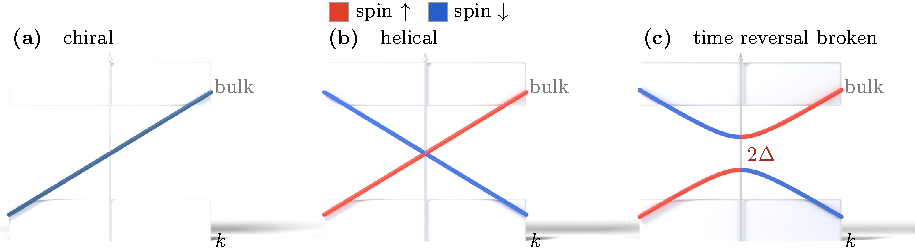
\includegraphics{figures/pdf/s03f06_helical.pdf}
\end{aqmfigure}


Disorder makes the distinction concrete: helical edge states survive disorder that preserves
time-reversal symmetry (the band structure is modified but the gapless crossing at the edge remains),
while disorder that breaks time-reversal symmetry opens a genuine gap in the edge spectrum and
destroys the protection entirely.

\begin{notebookbox}{\texttt{session3.ipynb}, ``The quantum spin Hall state'' (Core), ``The robustness of the quantum spin Hall state'' (Core), ``Topological invariant of the quantum spin Hall state'', and ``Finite size effects in topological systems'' (Challenge, using exchange coupling plus Rashba spin-orbit coupling)}
Build the two-copies-of-a-Chern-insulator model and identify the helical pair of edge states by
spin projection and propagation direction, exactly the pattern in (3.9). Then add disorder that
preserves versus breaks time-reversal symmetry and confirm the gap only opens in the second case.
The ``in the lab'' note in this notebook section points to the 1T$'$-WTe$_2$ measurement mentioned
above.
\end{notebookbox}

\section{Topology beyond electrons}

We built all of today's machinery, the Chern number, the Zak phase, the bulk-boundary
correspondence, around electronic band structures. None of the underlying mathematics actually
requires electrons. The same invariants apply to any quantum excitation with a well-defined
dispersion relation: \textbf{magnons}, the spin-wave excitations of an ordered magnet, and \textbf{spinons},
the fractionalized spin excitations of a quantum magnet, both admit exactly the same
Berry-curvature-and-Chern-number treatment, and we will carry it out explicitly for magnon bands in
session 6 and for spinon bands in session 8. More broadly still, the argument only needed a
Hamiltonian, or more generally a matrix describing how a wave propagates, so it applies to any system
with a dispersion relation at all: photonic systems (light propagating through a periodic medium),
and even purely classical mechanical systems, coupled pendula, vibrating lattices, electronic
circuits, have all been shown, in tabletop experiments, to host topologically protected modes.
Topology, in the end, is a statement about the internal structure of eigenvectors as a function of
momentum, and that structure exists wherever a wave equation does, quantum or not.

If there is one thing to take away from today, it is this: topological systems have protected edge
modes, those modes are tied to a non-trivial value of a topological invariant computed entirely from
the bulk, and this happens in both one and two dimensions (and beyond), typically protected by a
specific symmetry, translational symmetry and gauge invariance for the Chern number, time-reversal
symmetry for the quantum spin Hall state.

\section{Closing summary}

\begin{itemize}
\item The Hall conductivity, computed via linear response theory from the wavefunction expansion (3.1),
  reduces to an integral of the Berry curvature over the Brillouin zone and is quantized to an
  integer, the \textbf{Chern number}, for any gapped system: $\sigma_{xy} = C\,e^2/h$ (3.4).
\item The quantum Hall state realizes this with flat Landau-level bands, each contributing Chern number
  $1$; the bulk gap forces the current onto \textbf{chiral} edge states, one direction per edge, which is
  why they cannot backscatter and why the plateaus are so sharply quantized (Section 3.6).
\item \textbf{Topology} classifies Hamiltonians by whether their band structures can be continuously deformed
  into one another without closing the gap; the Chern number is that classification's invariant, and
  an interface between regions of different Chern number is forced to host a gapless state, the
  general \textbf{bulk-boundary correspondence} (Section 3.7).
\item The \textbf{SSH model} is the minimal one-dimensional realization: a $2\times 2$ Bloch Hamiltonian (3.5)
  whose lower-band Zak phase (3.6) is $0$ (trivial) or $\pi$ (topological) depending on whether the
  intracell hopping is larger or smaller than the intercell hopping, with the topological phase
  hosting protected zero-energy modes at the chain's ends.
\item A lattice hosting a \textbf{massive Dirac equation} (3.7) contributes Chern number $\tfrac12\,
  \mathrm{sgn}(m)\,\mathrm{sgn}(\lambda)$ per Dirac point (3.8); whether the contributions from
  time-reversal-paired Dirac points cancel or add depends entirely on how the mass term transforms
  under time reversal, which is exactly what separates a trivial gap (staggered sublattice potential)
  from a genuine \textbf{Chern insulator} (the Haldane model), the answer to the session's opening
  question of what happens when you gap the honeycomb Dirac cone.
\item Pairing two oppositely-massed copies of (3.7), one per spin, preserves time-reversal symmetry
  ($C=0$) while keeping a non-trivial spin Chern number $C_s=\pm2$ (3.9): the \textbf{quantum spin Hall
  insulator}, with helical edge states protected by Kramers degeneracy rather than by broken
  symmetry.
\item The same invariants generalize beyond electrons entirely, to magnons and spinons (sessions 6 and
  8), and beyond quantum mechanics altogether, to any system with a dispersion relation.
\end{itemize}

Next session we go back to the flat-band archetype from session 2 and work through it properly: the
full quantum Hall effect, Landau levels from first principles, and the fractional quantum Hall state.
